\documentclass[11pt]{article}
\usepackage{fullpage}
\usepackage{url}
\usepackage{amsmath, comment, graphicx, mathtools}
\usepackage{algorithm2e}
\usepackage[colorlinks=true,urlcolor=blue]{hyperref}
\usepackage{tikz}
\newcommand{\indep}{\rotatebox[origin=c]{90}{$\models$}}

\tikzset{
  treenode/.style = {shape=rectangle, rounded corners,
                     draw, align=center,
                     top color=white, bottom color=blue!20},
  root/.style     = {treenode, font=\Large, bottom color=red!30},
  env/.style      = {treenode, font=\ttfamily\normalsize},
  dummy/.style    = {circle,draw}
}

\begin{document}
\thispagestyle{empty}
\parindent 0pt
\vfill
\large

\title{GR5261 Report Scratch}
\author{Zhanhao Zhang}

\maketitle

\begin{algorithm}[H]
\hrulefill

\caption{Clustering Minimum Correlated Stocks}
\KwData{SP500 $STOCKS$ with their daily closing $PRICES$, cluster size $SIZE$}

Compute the absolute correlation matrix $COR_MATRIX$ among $STOCKS$\;
Find the pair ($STOCK1$, $STOCK2$) with least absolute correlation\;
Set $CLUSTER = [STOCK1$, $STOCK2]$\;
\While{$CLUSTER.size < SIZE$}{
	\For{$s$ in $STOCKS$}{
		\If{$s$ not in $CLUSTER$}{
			Set $CorWithCluster$ = 0\;
			\For{$s2$ in $CLUSTER$}{
				$CorWithCluster$ = $\max(CorWithCluster, COR_MATRIX[s, s2])$\;
			}
		}
	}
	Find $s$ with MINIMUM $CorWithCluster$\;
	Append $s$ to $CLUSTER$\;
}
\Return $CLUSTER$\;
\hrulefill
\end{algorithm}

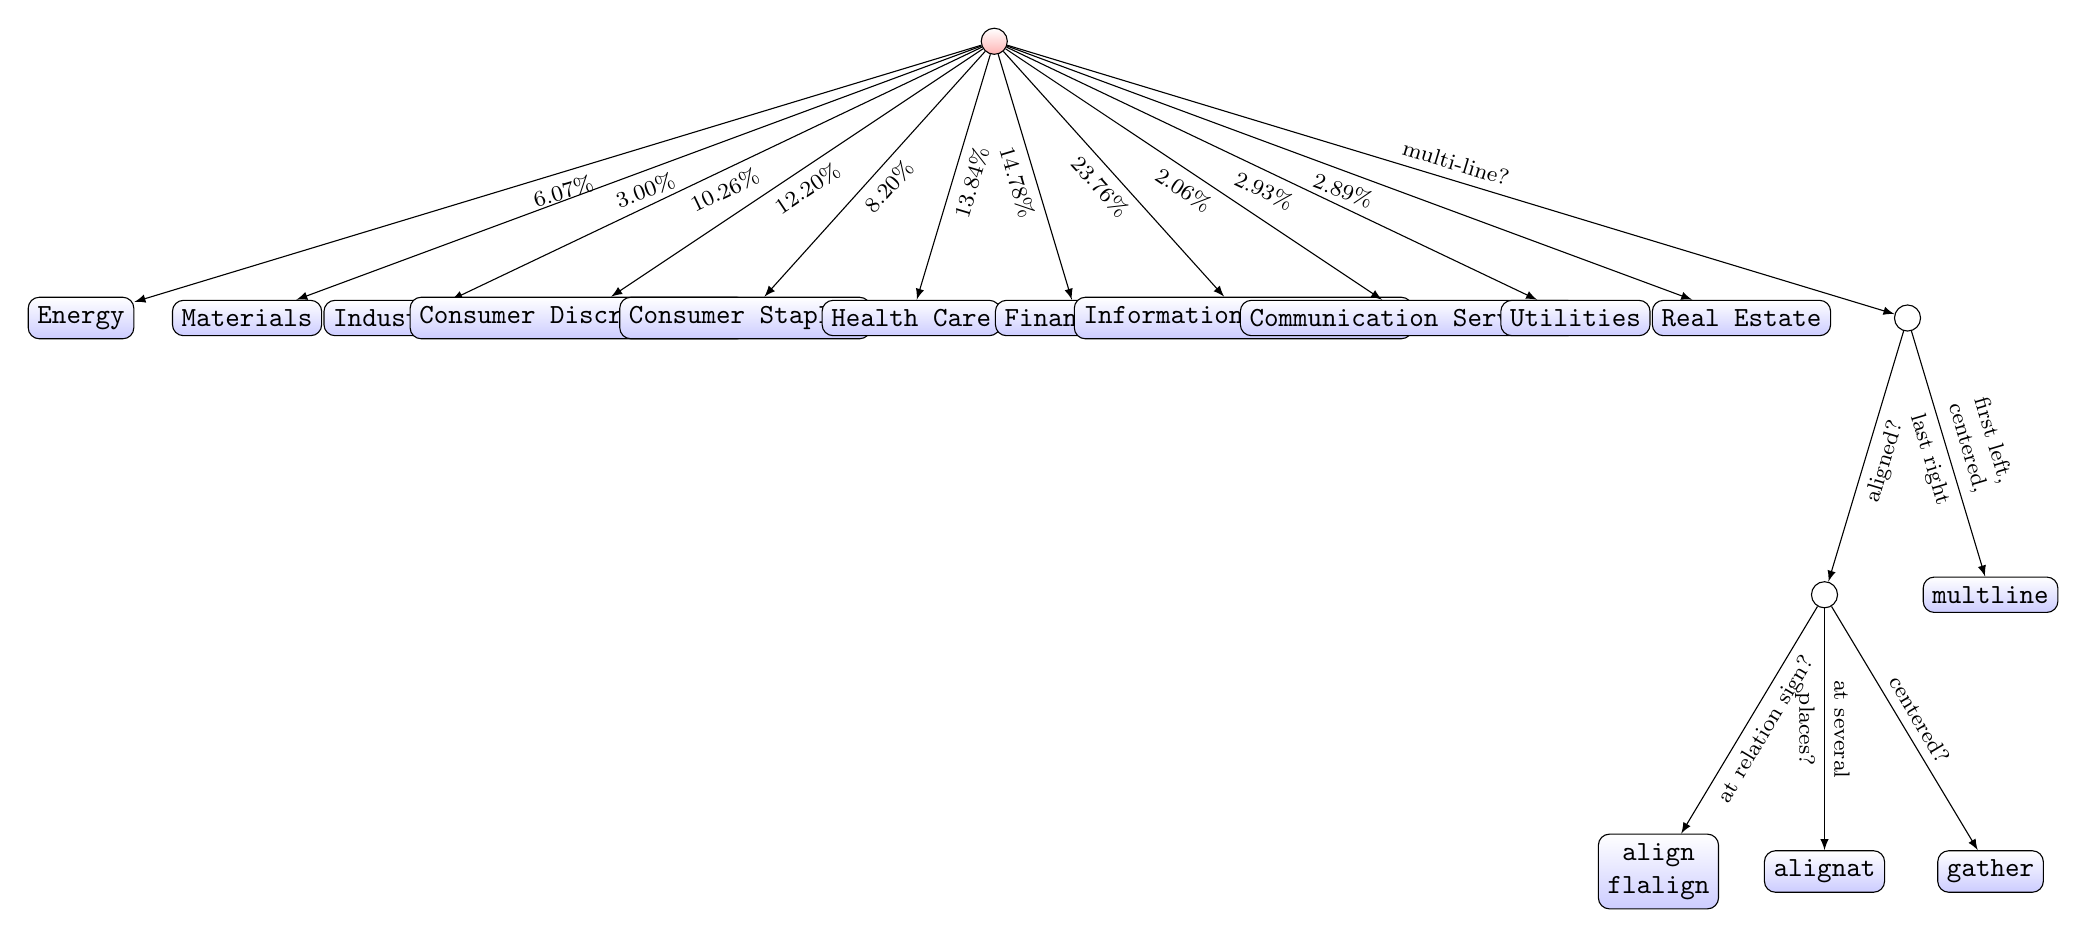
\begin{tikzpicture}
  [
    grow                    = down,
    sibling distance        = 6em,
    level distance          = 10em,
    edge from parent/.style = {draw, -latex},
    every node/.style       = {font=\footnotesize},
    sloped
  ]
  \node [root] [dummy] {}
    child { node [env] {Energy}
      edge from parent node [below] {6.07\%} }
    child { node [env] {Materials}
      edge from parent node [below] {3.00\%} }
    child { node [env] {Industrials}
      edge from parent node [below] {10.26\%} }
    child { node [env] {Consumer Discretionary}
      edge from parent node [below] {12.20\%} }
    child { node [env] {Consumer Staples}
      edge from parent node [below] {8.20\%} }
    child { node [env] {Health Care}
      edge from parent node [below] {13.84\%} }
    child { node [env] {Financials}
      edge from parent node [below] {14.78\%} }
    child { node [env] {Information Technology}
      edge from parent node [below] {23.76\%} }
    child { node [env] {Communication Services}
      edge from parent node [below] {2.06\%} }
    child { node [env] {Utilities}
      edge from parent node [below] {2.93\%} }
    child { node [env] {Real Estate}
      edge from parent node [below] {2.89\%} }
    child { node [dummy] {}
      child { node [dummy] {}
        child { node [env] {align\\flalign}
          edge from parent node [below] {at relation sign?} }
        child { node [env] {alignat}
          edge from parent node [above] {at several}
                           node [below] {places?} }
        child { node [env] {gather}
                edge from parent node [above] {centered?} }
        edge from parent node [below] {aligned?} }
      child { node [env] {multline}
              edge from parent node [above, align=center]
                {first left,\\centered,}
              node [below] {last right}}
              edge from parent node [above] {multi-line?} };
\end{tikzpicture}

\end{document}